\section{Wohlstandsverteilung und Umverteilung}

\subsection{Grundproblem der Verteilung}

Neben Wirtschaftswachstum gehört der \textbf{soziale Ausgleich} zu den zentralen Zielen der Wirtschaftspolitik.

Die zentrale Frage lautet:

\begin{itemize}
\item Wie wird der erzeugte Wohlstand in einer Volkswirtschaft verteilt?
\item Wie gross soll die staatliche Umverteilung sein?
\item Wie lässt sich soziale Gerechtigkeit mit Leistungsanreizen vereinbaren?
\end{itemize}

Umverteilung bedeutet, dass ein Teil des Wohlstands von einer Person oder Gruppe zu einer anderen transferiert wird.

\subsection{Effizienz und Verteilung}

Aus Sicht der Wirtschaftspolitik steht Verteilung im Spannungsfeld zwischen zwei Zielen:

\begin{itemize}
\item \textbf{Effizienz:} Gesamtwohlstand maximieren
\item \textbf{Gerechtigkeit:} gesellschaftlich akzeptable Verteilung
\end{itemize}

Ein wichtiger Effizienzbegriff ist die \textbf{Pareto-Effizienz}.

Eine Situation ist Pareto-effizient, wenn sich die Lage einer Person nur verbessern lässt, wenn sich gleichzeitig die Lage einer anderen Person verschlechtert.

\textbf{Grundidee:}

Zuerst Wohlstand vergrössern, danach verteilen.

\subsection{Zielkonflikt zwischen Effizienz und Umverteilung}

Zwischen Effizienz und Verteilung besteht ein Zielkonflikt.

\begin{itemize}
\item Zu starke Umverteilung reduziert Leistungsanreize
\item Zu geringe Umverteilung wird gesellschaftlich als ungerecht empfunden
\end{itemize}

Die Herausforderung der Wirtschaftspolitik besteht darin, ein Gleichgewicht zwischen diesen beiden Zielen zu finden.

\subsection{Messung der Ungleichheit}

\begin{center}
    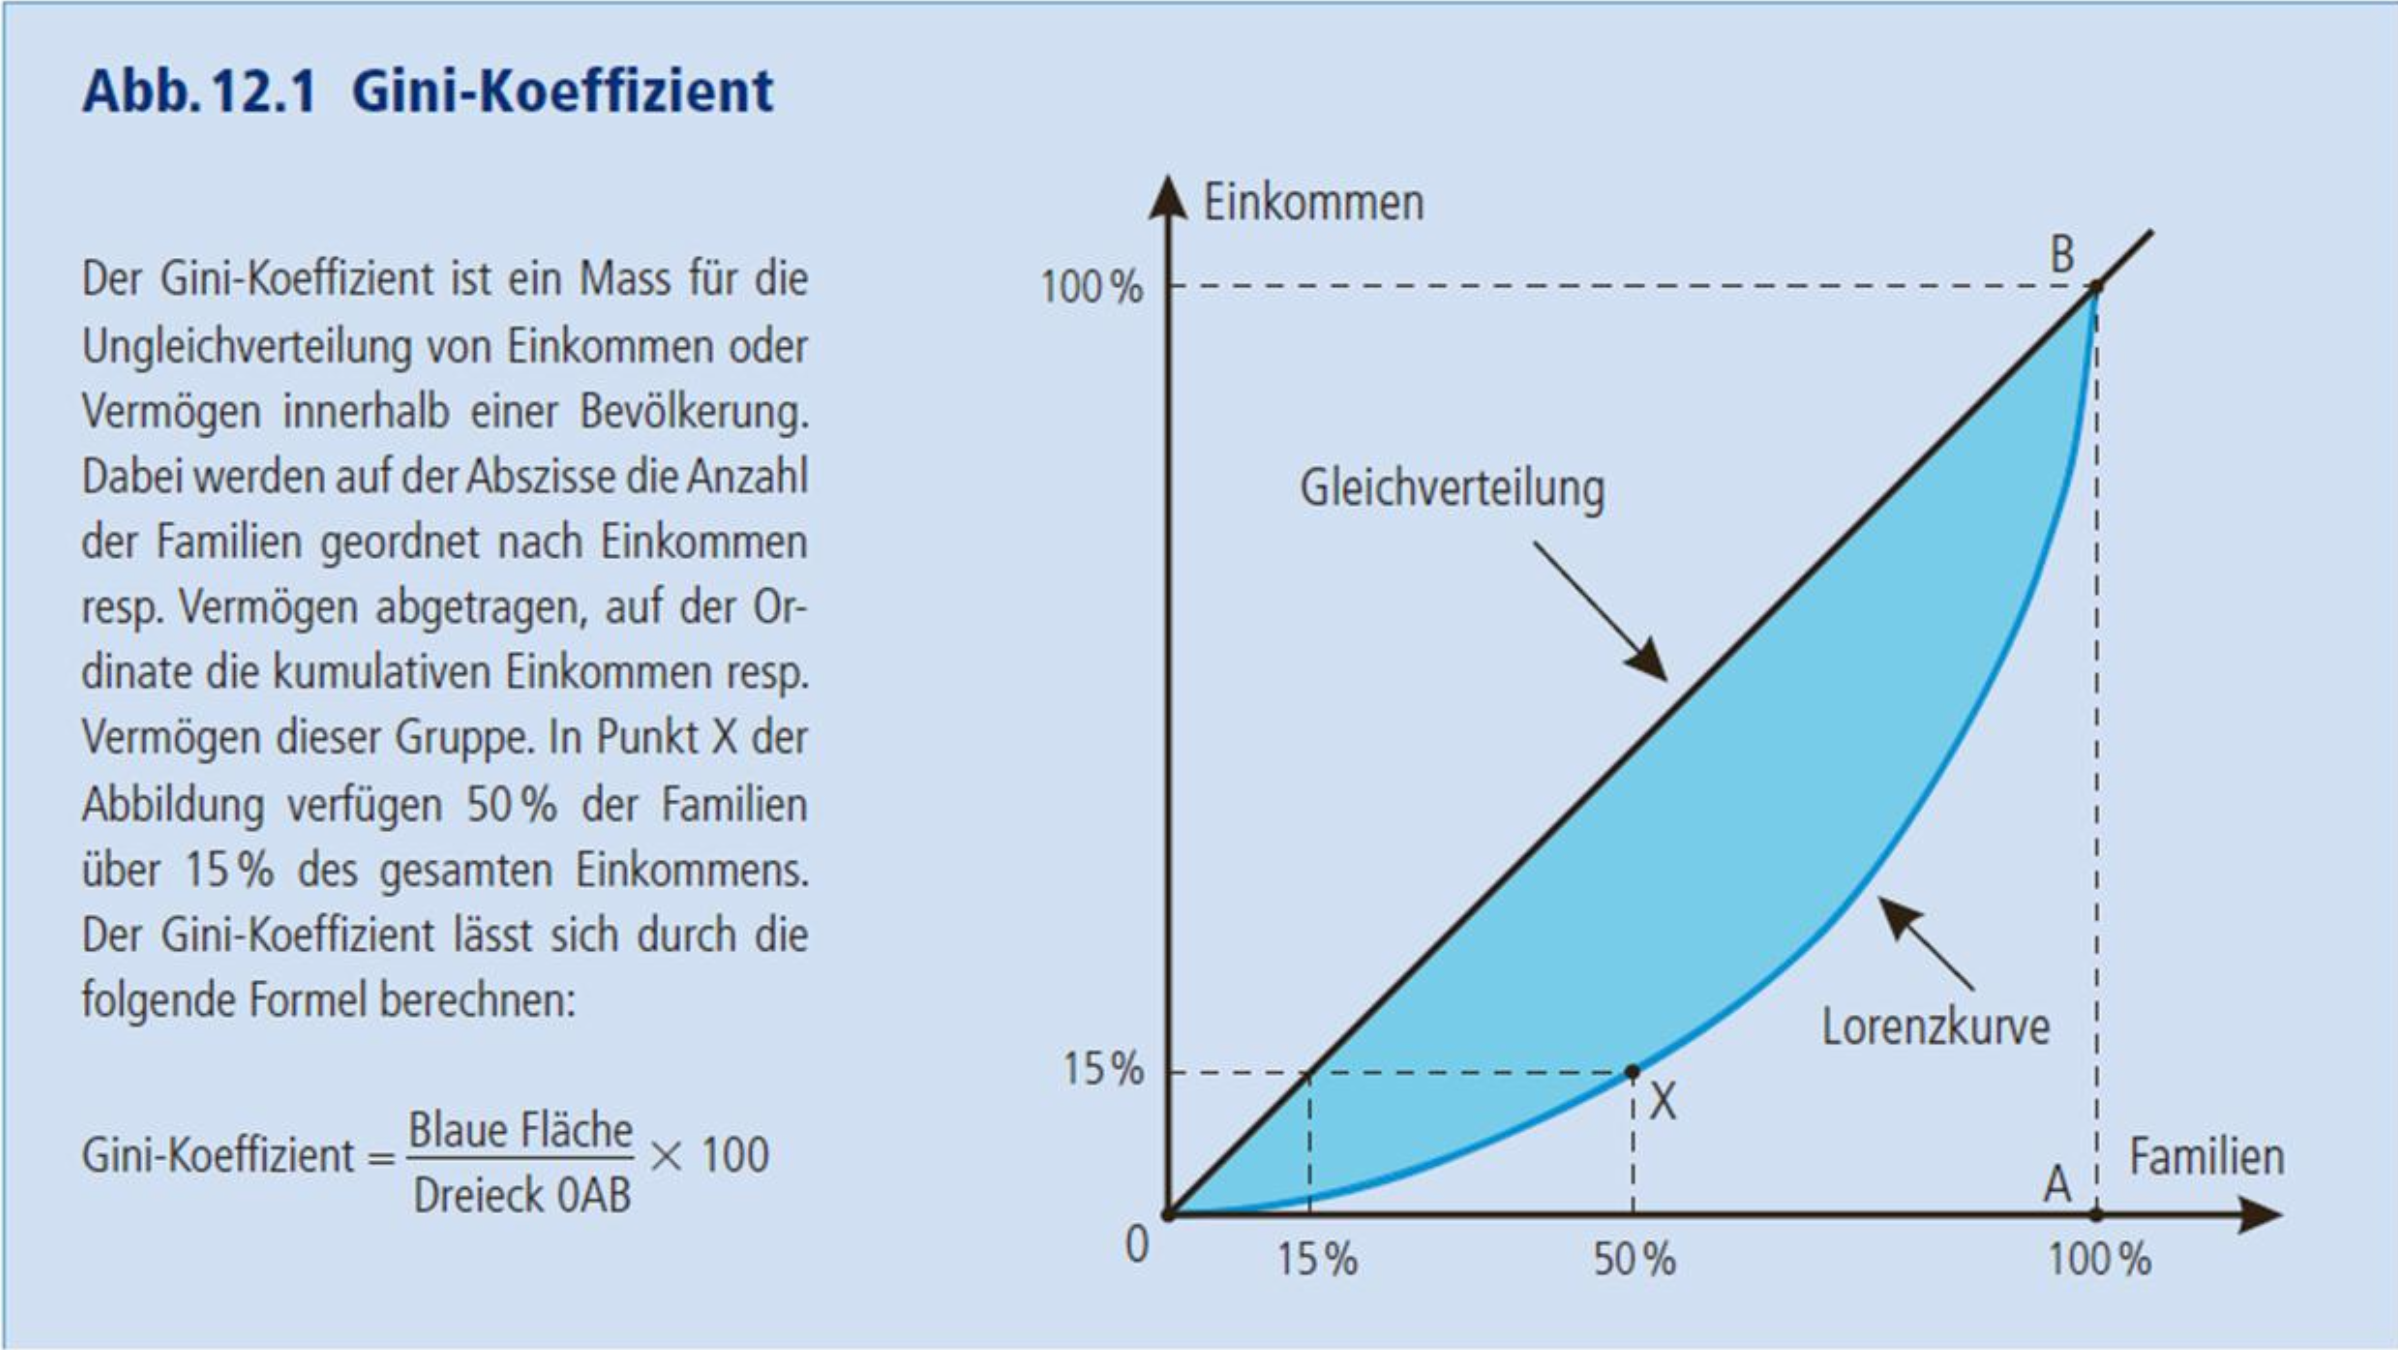
\includegraphics[width=0.5\linewidth]{images/lorenzkurve.png} 
\end{center}

Die Verteilung von Einkommen oder Vermögen wird mit zwei zentralen Instrumenten gemessen.

\subsubsection{Lorenzkurve}

Die Lorenzkurve stellt die kumulative Einkommensverteilung dar.

\begin{itemize}
\item Horizontale Achse: Anteil der Bevölkerung
\item Vertikale Achse: Anteil des Einkommens
\end{itemize}

Bei perfekter Gleichverteilung gilt:

\[
20\% \text{ der Bevölkerung besitzen } 20\% \text{ des Einkommens}
\]

Je stärker die Lorenzkurve von der Gleichverteilungslinie abweicht, desto ungleicher ist die Verteilung.

\subsubsection{Gini-Koeffizient}

Der Gini-Koeffizient misst die Ungleichheit der Verteilung.

\[
Gini = \frac{\text{Fläche zwischen Gleichverteilung und Lorenzkurve}}
{\text{Gesamtfläche unter der Gleichverteilung}}
\]

Eigenschaften:

\begin{itemize}
\item $0$ = vollständige Gleichverteilung
\item $1$ = maximale Ungleichverteilung
\end{itemize}

\subsection{Einkommensverteilung weltweit}

\begin{center}
    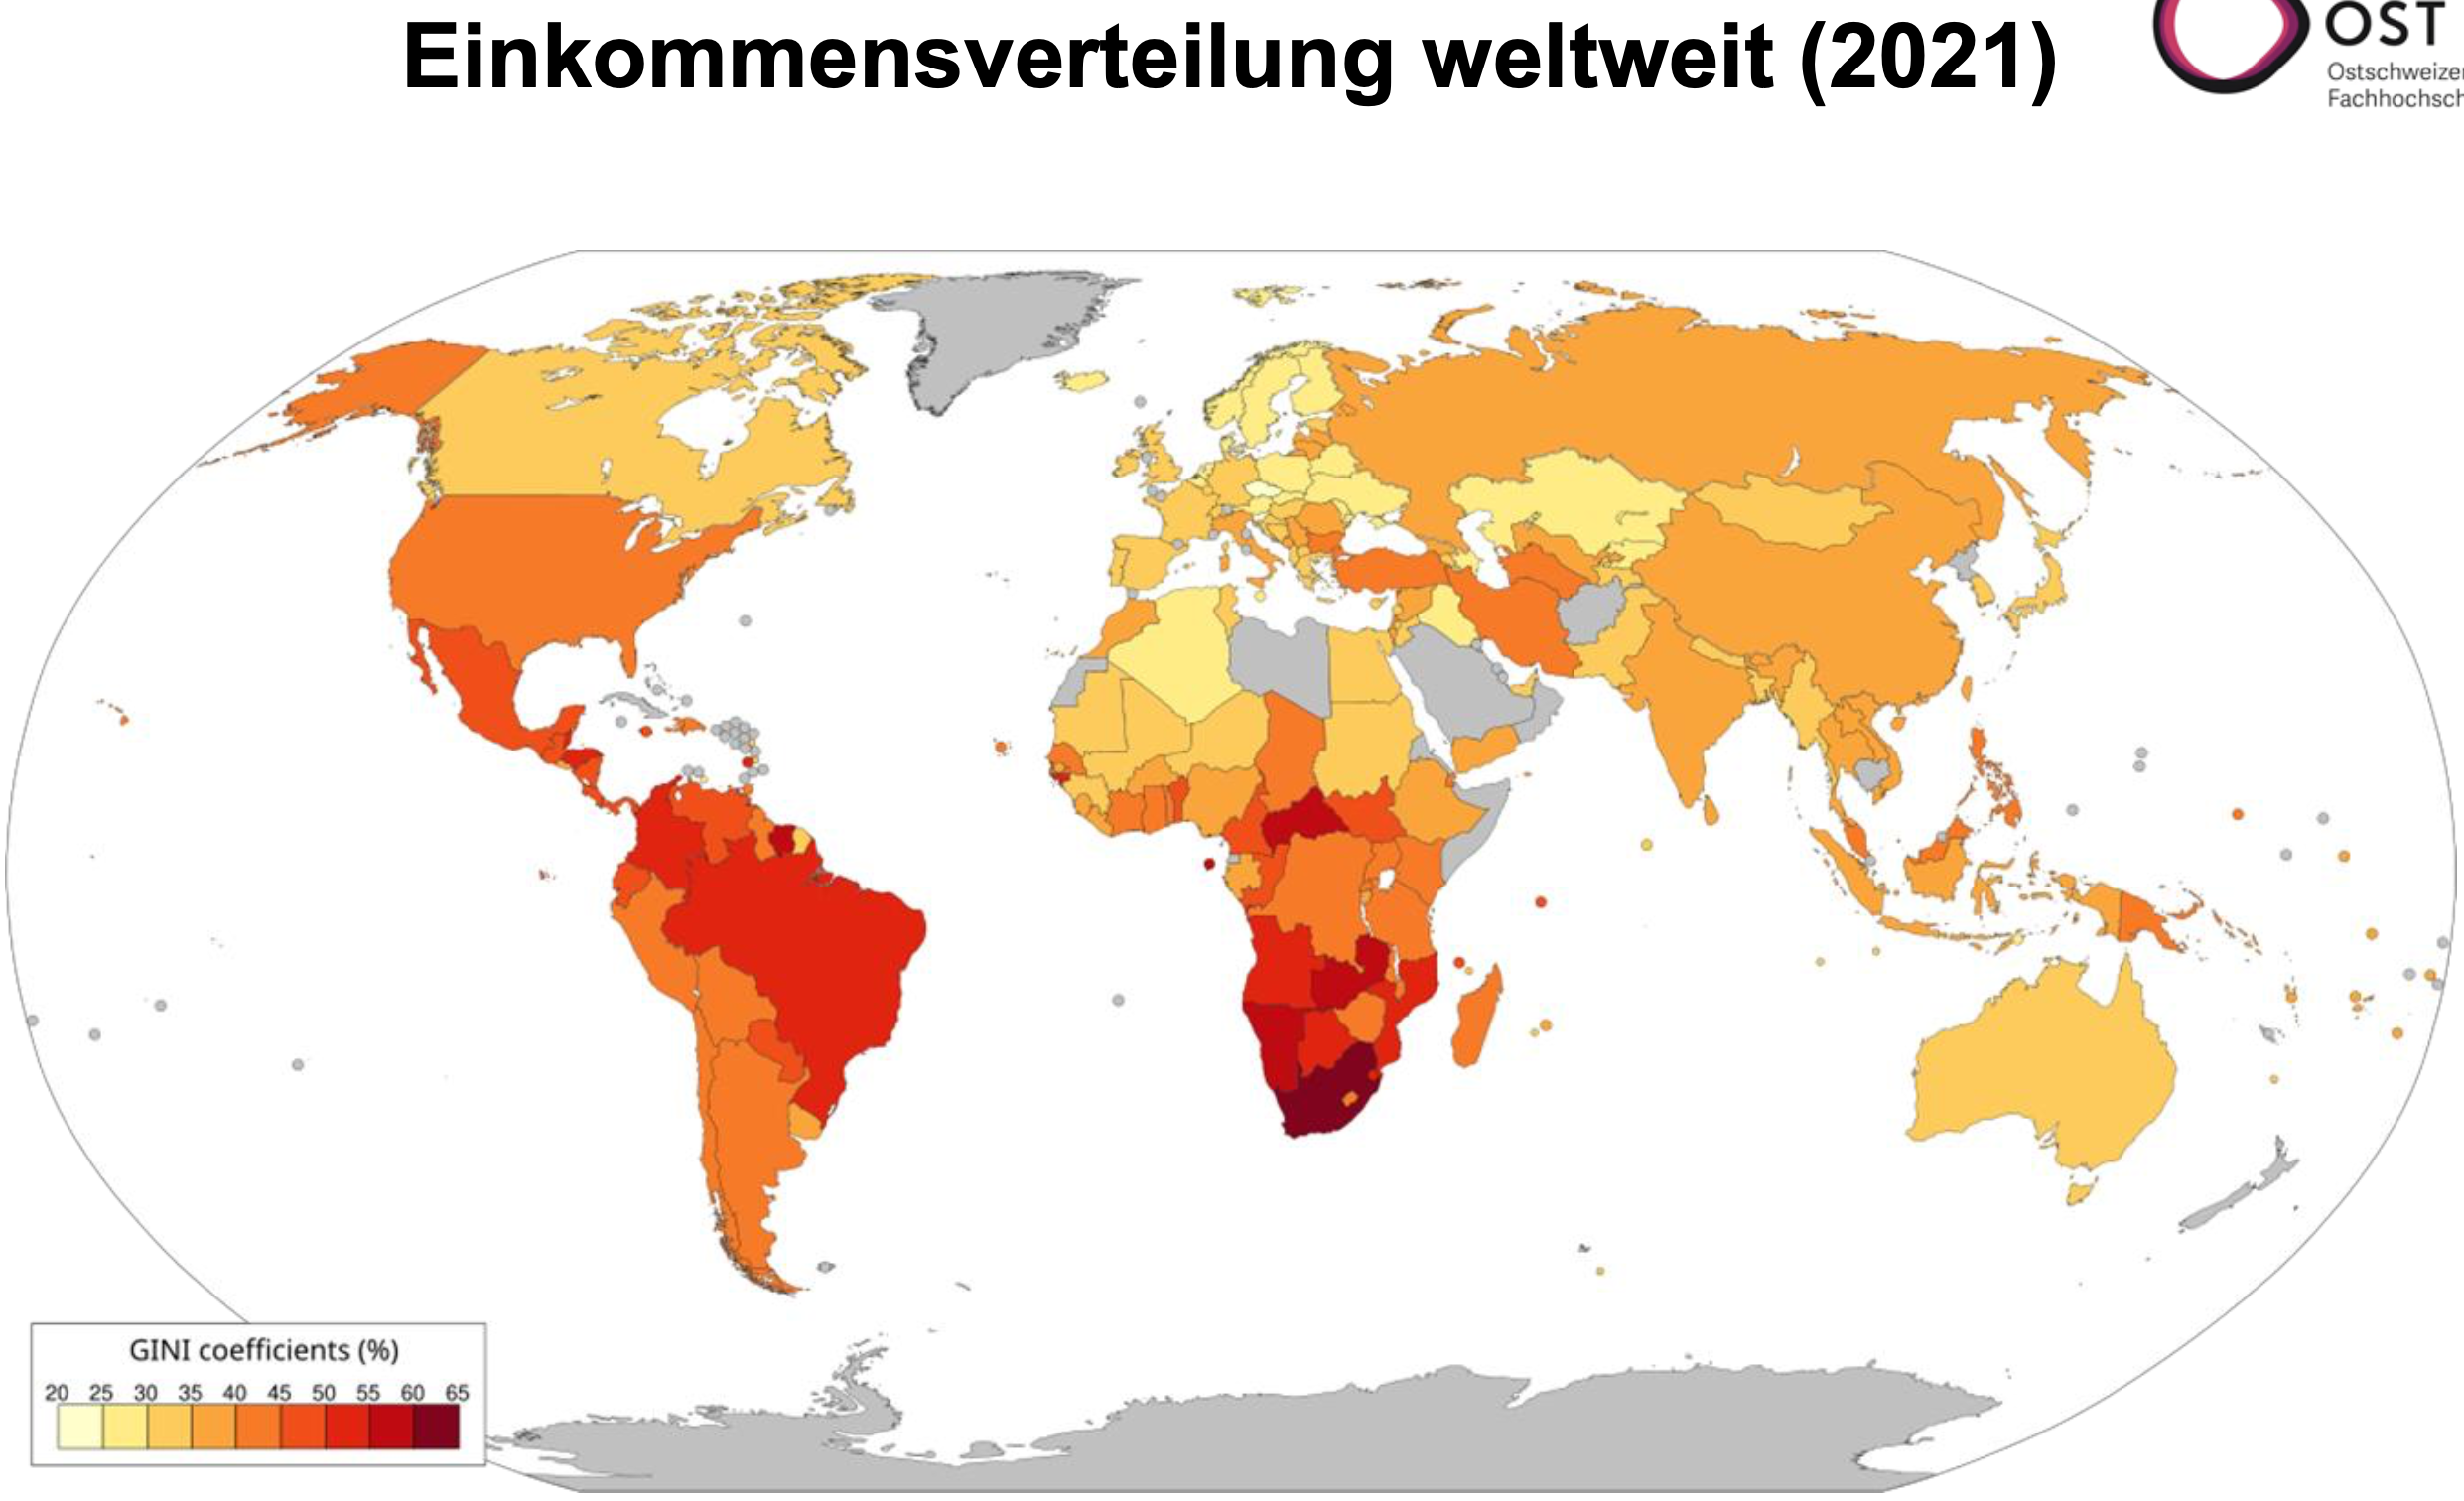
\includegraphics[width=0.7\linewidth]{images/einkommensverteilung.png}
\end{center}

Die Einkommensverteilung unterscheidet sich stark zwischen Ländern.

Typische Beobachtungen:

\begin{itemize}
\item Industrieländer weisen meist geringere Ungleichheit auf
\item Schwellenländer oft deutlich höhere Ungleichheit
\item Staatliche Umverteilung reduziert Ungleichheit
\end{itemize}

\subsection{Vermögensverteilung weltweit}
\begin{center}
    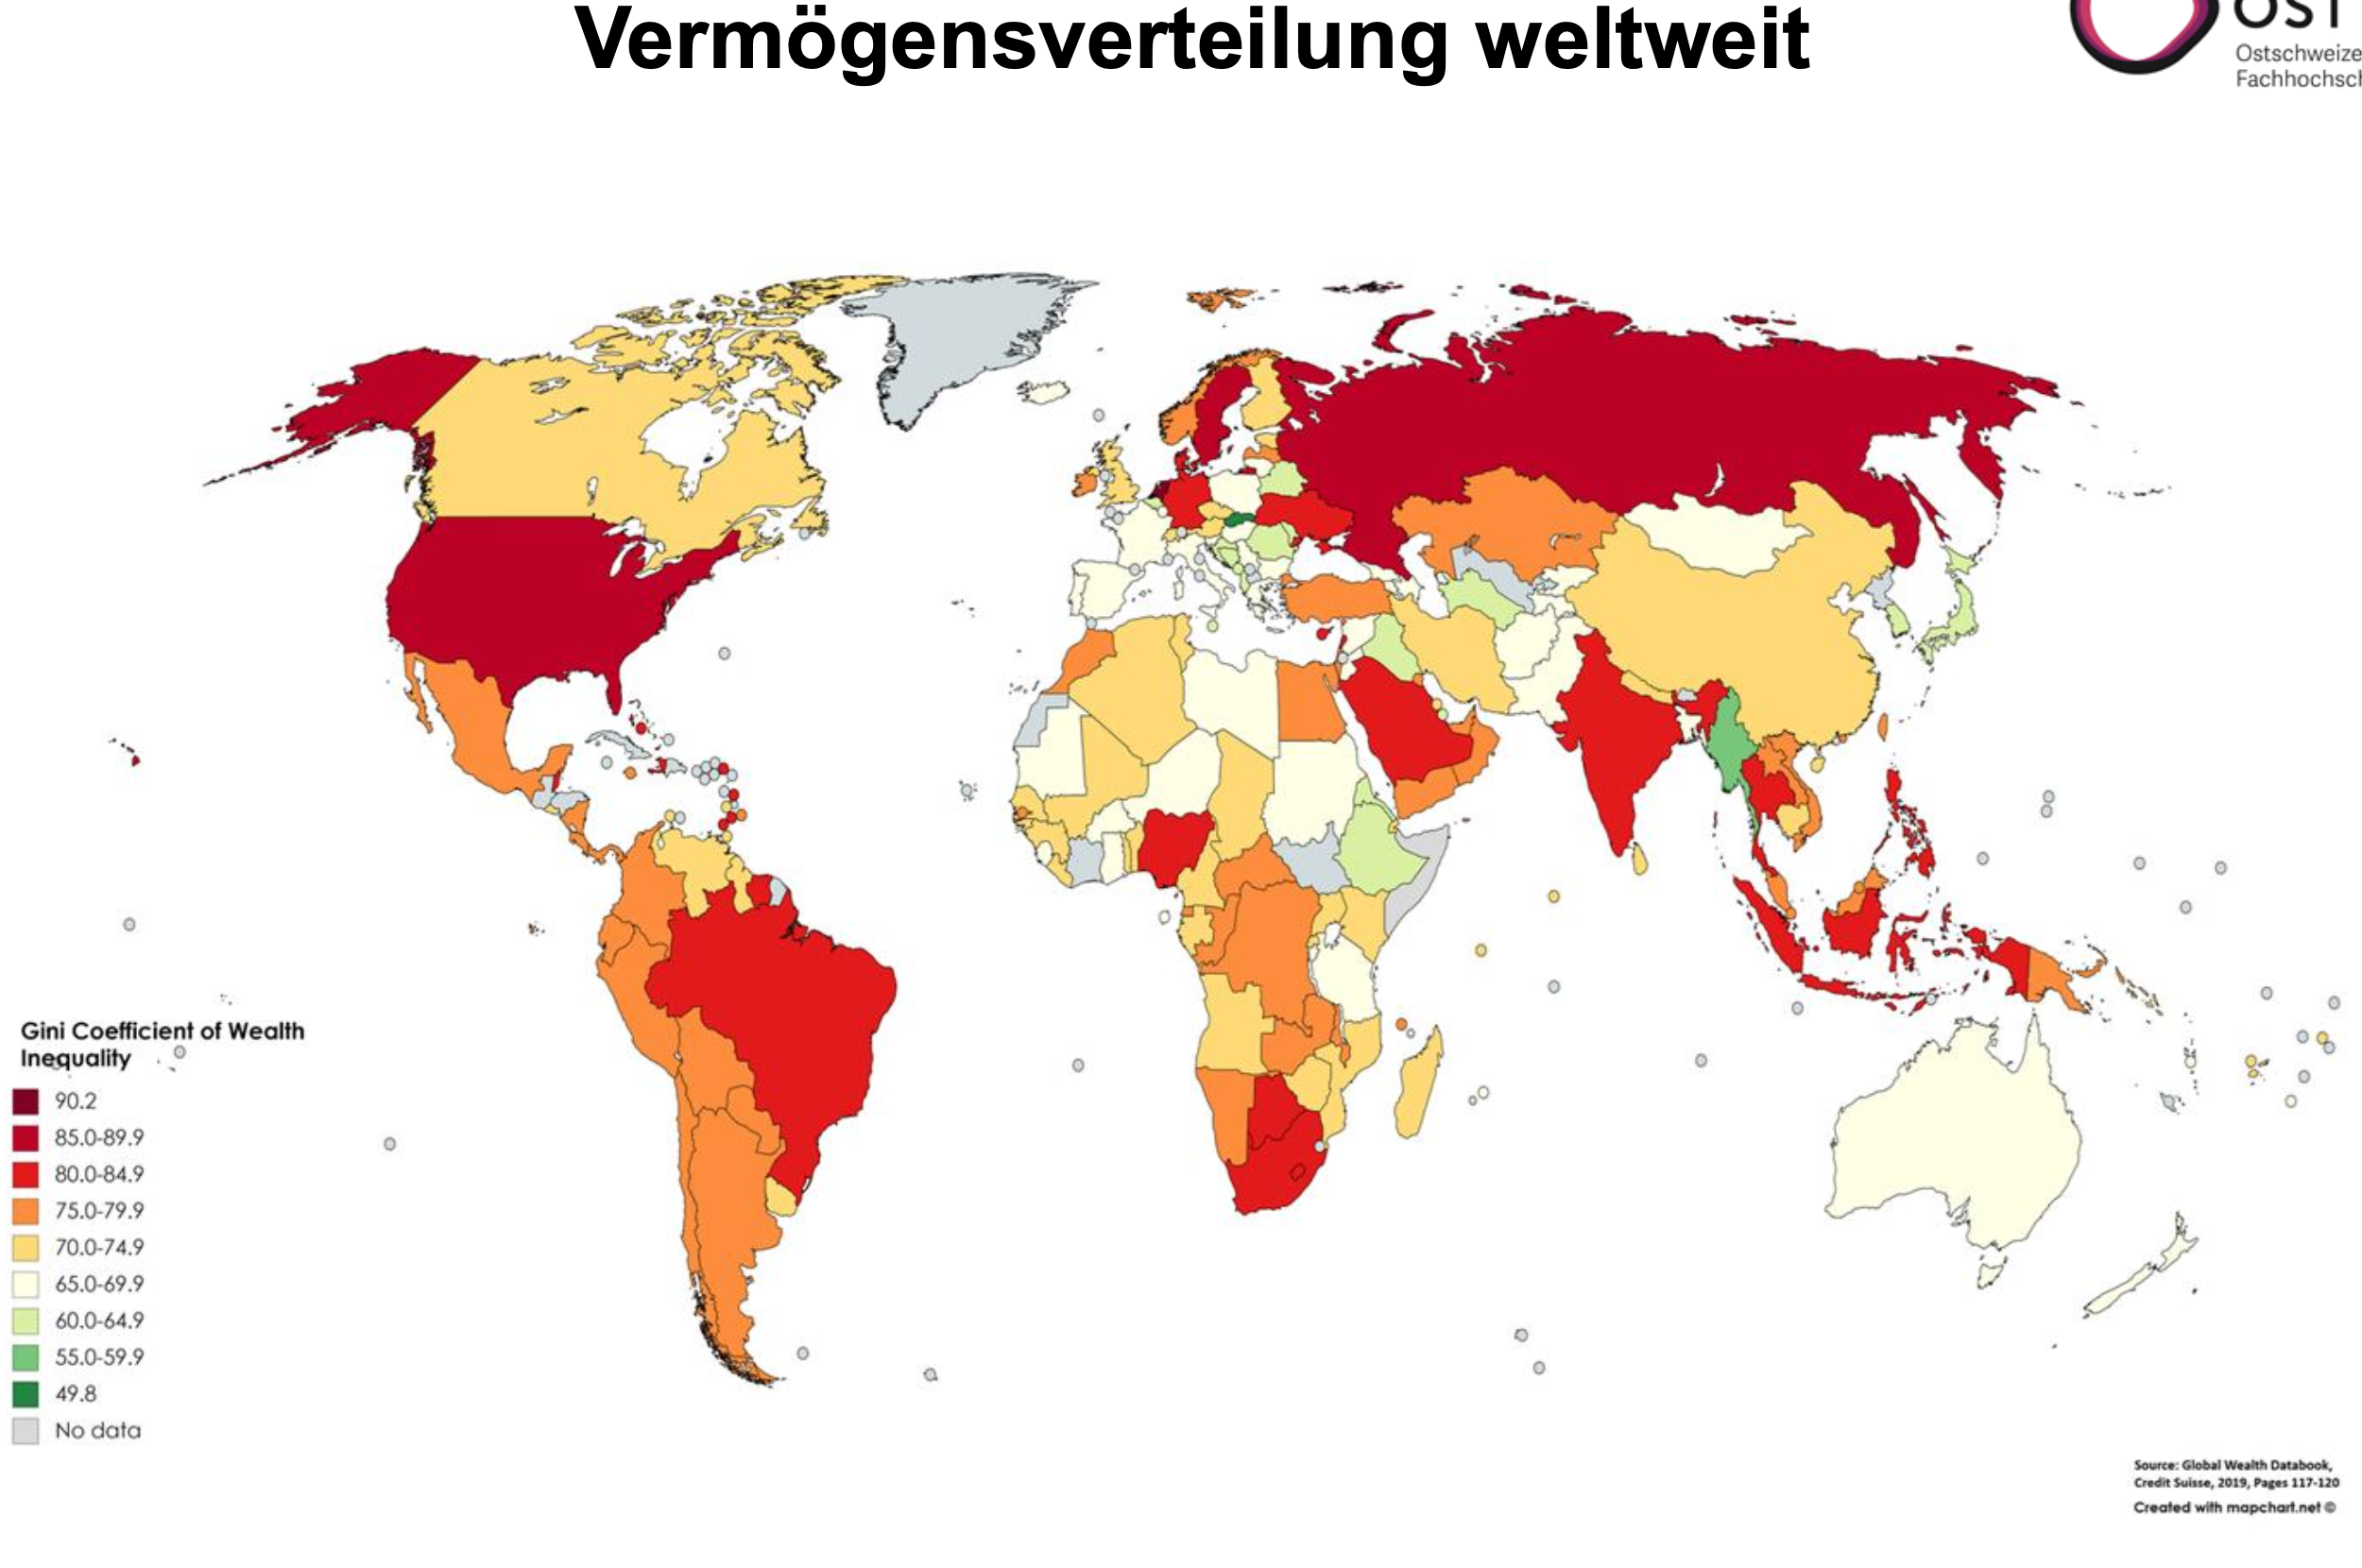
\includegraphics[width=0.7\linewidth]{images/vermögensverteilung.png}
\end{center}

Vermögen ist weltweit deutlich ungleicher verteilt als Einkommen.

Häufige Ursachen:

\begin{itemize}
\item Kapitalerträge
\item Erbschaften
\item langfristige Vermögensakkumulation
\end{itemize}

\subsection{Vermögensverteilung in der Schweiz}

\begin{center}
    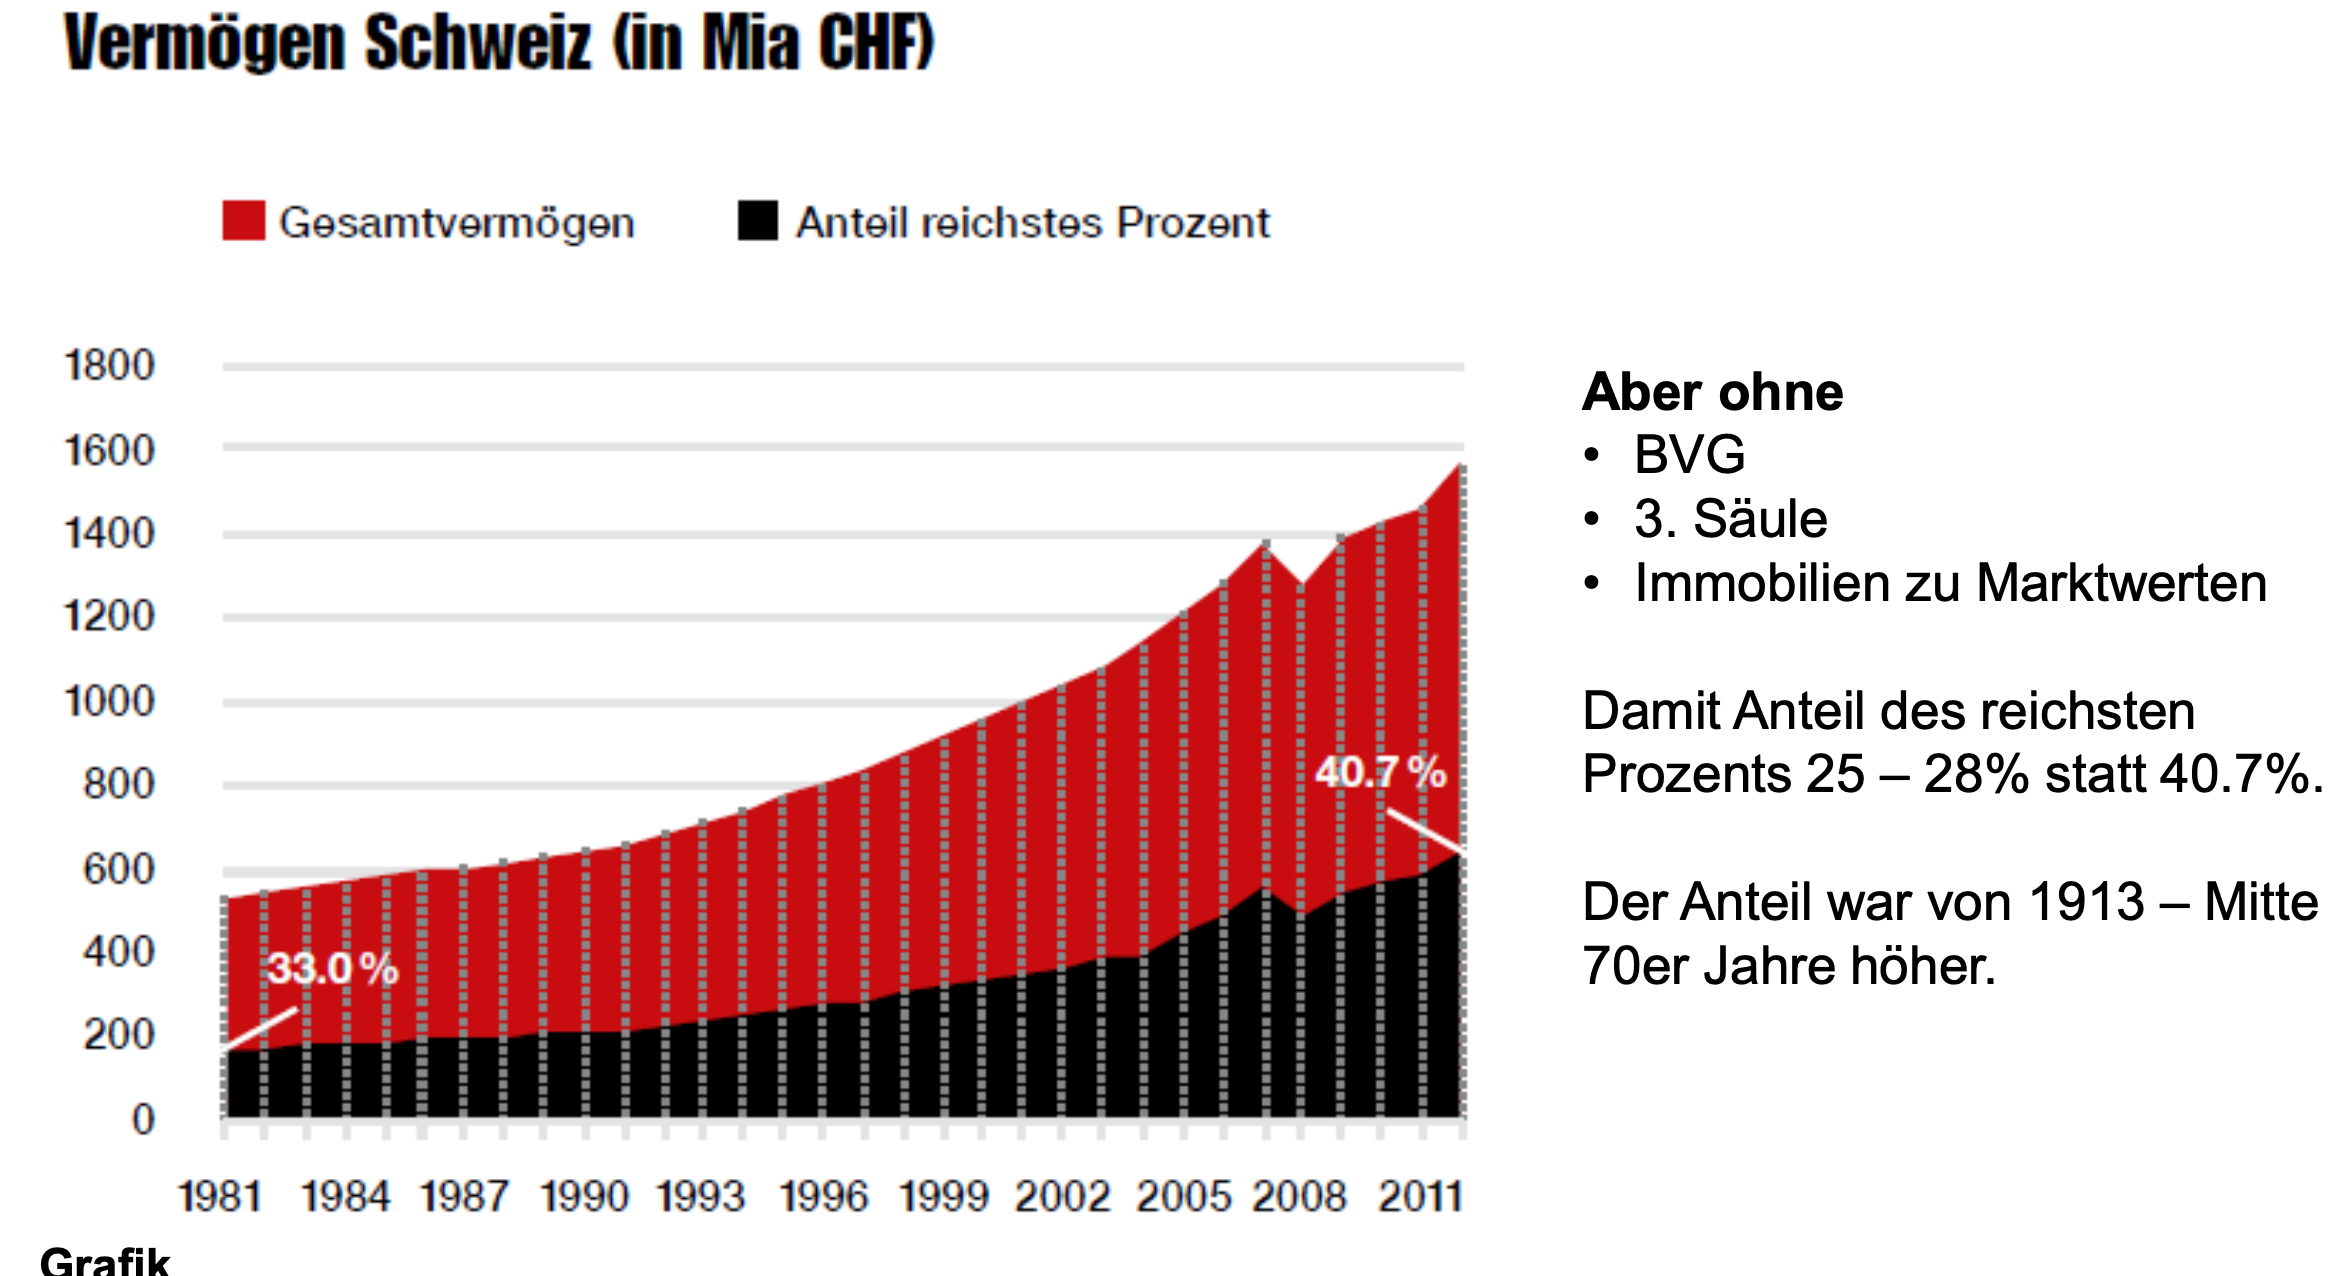
\includegraphics[width=0.7\linewidth]{images/vermoegen_schweiz.png}
\end{center}

Auch in der Schweiz ist Vermögen sehr ungleich verteilt.

Studien zeigen:

\begin{itemize}
\item Das reichste Prozent besitzt einen sehr grossen Anteil des Vermögens
\item Der Gini-Koeffizient für Vermögen ist sehr hoch
\end{itemize}

Je nach Berechnung liegt der Anteil des reichsten Prozents am Gesamtvermögen zwischen etwa 25\% und über 40\%.

\subsection{Einkommensquellen}

Einkommen kann aus verschiedenen Quellen stammen:

\begin{itemize}
\item Arbeitseinkommen (Lohn)
\item Vermögenseinkommen (Zinsen, Dividenden)
\item Staatliche Transfers
\end{itemize}

Diese bilden die Grundlage für staatliche Umverteilung.

\subsection{Instrumente der Umverteilung}

Der Staat kann Umverteilung über zwei Wege durchführen.

\subsubsection{Umverteilung über Einnahmen}

\begin{itemize}
\item Progressive Einkommenssteuer
\item Vermögenssteuer
\end{itemize}

Höhere Einkommen zahlen überproportional höhere Steuern.

\subsubsection{Umverteilung über Ausgaben}

\begin{itemize}
\item Direkte Geldtransfers
\item Subventionierte staatliche Leistungen
\end{itemize}

Beispiele:

\begin{itemize}
\item Sozialhilfe
\item Prämienverbilligungen
\item Familienzulagen
\end{itemize}

\subsection{Umverteilung in der Schweiz}

Im internationalen Vergleich weist die Schweiz:

\begin{itemize}
\item relativ geringe Einkommensungleichheit
\item moderate staatliche Umverteilung
\end{itemize}

Der Unterschied zwischen Markt- und Nettoeinkommen zeigt die Wirkung staatlicher Umverteilung.

\subsection{Die Sozialwerke der Schweiz}

Ein grosser Teil der Umverteilung erfolgt über die Sozialversicherungen.

Wichtige Sozialwerke:

\begin{itemize}
\item AHV (Alters- und Hinterlassenenversicherung)
\item IV (Invalidenversicherung)
\item ALV (Arbeitslosenversicherung)
\item BVG (berufliche Vorsorge)
\item Krankenversicherung
\end{itemize}

Diese sichern verschiedene Lebensrisiken ab:

\begin{itemize}
\item Alter
\item Krankheit
\item Arbeitslosigkeit
\item Invalidität
\end{itemize}

\subsection{Das Drei-Säulen-System der Altersvorsorge}

Die Altersvorsorge in der Schweiz basiert auf drei Säulen.

\begin{enumerate}
\item AHV (staatliche Grundsicherung)
\item BVG / Pensionskasse (berufliche Vorsorge)
\item Private Vorsorge (3. Säule)
\end{enumerate}

Ziele:

\begin{itemize}
\item Sicherung des Existenzminimums
\item Fortsetzung des gewohnten Lebensstandards
\item Individuelle Zusatzvorsorge
\end{itemize}

\subsection{Demografische Entwicklung}

Die Altersstruktur der Bevölkerung verändert sich stark.

Tendenzen:

\begin{itemize}
\item steigende Lebenserwartung
\item sinkende Geburtenrate
\item alternde Bevölkerung
\end{itemize}

Folge:

\begin{itemize}
\item mehr Rentner
\item weniger Erwerbstätige pro Rentner
\end{itemize}

Dies stellt eine grosse Herausforderung für die Finanzierung der Sozialwerke dar.

\subsection{Politische Stellschrauben}

Die Politik kann verschiedene Parameter anpassen:

\begin{itemize}
\item Beitragssätze
\item Rentenhöhe
\item Rentenalter
\end{itemize}

Andere Faktoren sind nur indirekt beeinflussbar:

\begin{itemize}
\item Migration
\item Geburtenrate
\item Wirtschaftswachstum
\end{itemize}

\subsection{Bedingungsloses Grundeinkommen}

Eine alternative Idee der Umverteilung ist das \textbf{bedingungslose Grundeinkommen (BGE)}.

Grundprinzip:

Jede Person erhält unabhängig von Arbeit oder Einkommen einen festen Geldbetrag.

Vorgeschlagene Beträge in der Schweizer Initiative:

\begin{itemize}
\item Erwachsene: CHF 2500 pro Monat
\item Kinder: CHF 625 pro Monat
\end{itemize}

Finanzierung würde grosse Teile des Sozialstaates ersetzen und neue Steuern erfordern.

Die Initiative wurde 2016 in einer Volksabstimmung deutlich abgelehnt.

\subsection{Gesamtfazit}

Die Verteilung von Einkommen und Vermögen ist ein zentraler Bestandteil der Wirtschaftspolitik.

Wesentliche Erkenntnisse:

\begin{itemize}
\item Märkte erzeugen von Natur aus Ungleichheit
\item Staaten greifen durch Umverteilung ein
\item Sozialwerke sind das wichtigste Instrument der Umverteilung
\item Demografischer Wandel stellt eine zentrale Herausforderung dar
\end{itemize}